\documentclass[]{article}
\usepackage{lmodern}
\usepackage{amssymb,amsmath}
\usepackage{ifxetex,ifluatex}
\usepackage{fixltx2e} % provides \textsubscript
\ifnum 0\ifxetex 1\fi\ifluatex 1\fi=0 % if pdftex
  \usepackage[T1]{fontenc}
  \usepackage[utf8]{inputenc}
\else % if luatex or xelatex
  \ifxetex
    \usepackage{mathspec}
  \else
    \usepackage{fontspec}
  \fi
  \defaultfontfeatures{Ligatures=TeX,Scale=MatchLowercase}
\fi
% use upquote if available, for straight quotes in verbatim environments
\IfFileExists{upquote.sty}{\usepackage{upquote}}{}
% use microtype if available
\IfFileExists{microtype.sty}{%
\usepackage{microtype}
\UseMicrotypeSet[protrusion]{basicmath} % disable protrusion for tt fonts
}{}
\usepackage[margin=1in]{geometry}
\usepackage{hyperref}
\hypersetup{unicode=true,
            pdfborder={0 0 0},
            breaklinks=true}
\urlstyle{same}  % don't use monospace font for urls
\usepackage{graphicx,grffile}
\makeatletter
\def\maxwidth{\ifdim\Gin@nat@width>\linewidth\linewidth\else\Gin@nat@width\fi}
\def\maxheight{\ifdim\Gin@nat@height>\textheight\textheight\else\Gin@nat@height\fi}
\makeatother
% Scale images if necessary, so that they will not overflow the page
% margins by default, and it is still possible to overwrite the defaults
% using explicit options in \includegraphics[width, height, ...]{}
\setkeys{Gin}{width=\maxwidth,height=\maxheight,keepaspectratio}
\IfFileExists{parskip.sty}{%
\usepackage{parskip}
}{% else
\setlength{\parindent}{0pt}
\setlength{\parskip}{6pt plus 2pt minus 1pt}
}
\setlength{\emergencystretch}{3em}  % prevent overfull lines
\providecommand{\tightlist}{%
  \setlength{\itemsep}{0pt}\setlength{\parskip}{0pt}}
\setcounter{secnumdepth}{0}
% Redefines (sub)paragraphs to behave more like sections
\ifx\paragraph\undefined\else
\let\oldparagraph\paragraph
\renewcommand{\paragraph}[1]{\oldparagraph{#1}\mbox{}}
\fi
\ifx\subparagraph\undefined\else
\let\oldsubparagraph\subparagraph
\renewcommand{\subparagraph}[1]{\oldsubparagraph{#1}\mbox{}}
\fi

%%% Use protect on footnotes to avoid problems with footnotes in titles
\let\rmarkdownfootnote\footnote%
\def\footnote{\protect\rmarkdownfootnote}

%%% Change title format to be more compact
\usepackage{titling}

% Create subtitle command for use in maketitle
\providecommand{\subtitle}[1]{
  \posttitle{
    \begin{center}\large#1\end{center}
    }
}

\setlength{\droptitle}{-2em}

  \title{}
    \pretitle{\vspace{\droptitle}}
  \posttitle{}
    \author{}
    \preauthor{}\postauthor{}
    \date{}
    \predate{}\postdate{}
  

\begin{document}

\begin{verbatim}
## Warning: package 'tinytex' was built under R version 3.6.1
\end{verbatim}

\begin{verbatim}
## If reinstallation fails, try install_tinytex() again. Then install the following packages:
## 
## tinytex::tlmgr_install(c("amscls", "amsfonts", "amsmath", "babel", "biber", "biblatex", "bibtex", "bigfoot", "booktabs", "caption", "cm", "dehyph", "dejavu", "dvipdfmx", "dvips", "ec", "enumitem", "environ", "etex", "etoolbox", "euenc", "fancyhdr", "fancyvrb", "filehook", "fontawesome", "fontspec", "framed", "geometry", "glyphlist", "graphics", "graphics-cfg", "graphics-def", "gsftopk", "helvetic", "hyperref", "hyphen-base", "ifluatex", "ifmtarg", "iftex", "ifxetex", "inconsolata", "knuth-lib", "kpathsea", "l3kernel", "l3packages", "latex", "latex-bin", "latex-fonts", "latexconfig", "latexmk", "lm", "lm-math", "logreq", "lualibs", "luaotfload", "luatex", "makeindex", "mathspec", "metafont", "mfware", "microtype", "ms", "natbib", "oberdiek", "parskip", "pdftex", "pgf", "plain", "scheme-infraonly", "setspace", "sourcesanspro", "tcolorbox", "tetex", "tex", "tex-ini-files", "texlive.infra", "times", "tipa", "titling", "tlgs", "tlperl", "tlpsv", "tools", "trimspaces", "unicode-data", "unicode-math", "upquote", "url", "xargs", "xcolor", "xetex", "xetexconfig", "xifthen", "xkeyval", "xpatch", "xunicode", "zapfding"))
\end{verbatim}

\begin{verbatim}
## The directory C:\Users\matthew.grainger\AppData\Roaming\TinyTeX/texmf-local is not empty. It will be backed up to C:\Users\MATTHE~1.GRA\AppData\Local\Temp\RtmpG2F7Ge\file2c1832d17a7a and restored later.
\end{verbatim}

\begin{verbatim}
## tlmgr conf auxtrees remove "C:/Programs/R/R-36~1.0/share/texmf"
\end{verbatim}

\begin{verbatim}
## tlmgr path remove
\end{verbatim}

\begin{verbatim}
## Starting to install TinyTeX to C:\Users\matthew.grainger\AppData\Roaming\TinyTeX. It will take a few minutes.
\end{verbatim}

\begin{verbatim}
## Next you may see two error dialog boxes about the missing luatex.dll, and an error message like "Use of uninitialized value in bitwise or (|)..." in the end. These messages can be ignored.
\end{verbatim}

\begin{verbatim}
## Warning in file.copy(list.files("TinyTeX", full.names = TRUE), target,
## recursive = TRUE): problem copying TinyTeX\tlpkg\installer\tar.exe to C:
## \Users\matthew.grainger\AppData\Roaming\TinyTeX\tlpkg\installer\tar.exe:
## Permission denied
\end{verbatim}

\begin{verbatim}
## Warning in file.copy(list.files("TinyTeX", full.names
## = TRUE), target, recursive = TRUE): problem copying
## TinyTeX\tlpkg\tlperl\bin\libgcc_s_dw2-1.dll to C:
## \Users\matthew.grainger\AppData\Roaming\TinyTeX\tlpkg\tlperl\bin\libgcc_s_dw2-1.dll:
## Permission denied
\end{verbatim}

\begin{verbatim}
## Warning in file.copy(list.files("TinyTeX", full.names
## = TRUE), target, recursive = TRUE): problem copying
## TinyTeX\tlpkg\tlperl\bin\libstdc++-6.dll to C:
## \Users\matthew.grainger\AppData\Roaming\TinyTeX\tlpkg\tlperl\bin\libstdc+
## +-6.dll: Permission denied
\end{verbatim}

\begin{verbatim}
## Warning in file.copy(list.files("TinyTeX", full.names
## = TRUE), target, recursive = TRUE): problem copying
## TinyTeX\tlpkg\tlperl\bin\libwinpthread-1.dll to C:
## \Users\matthew.grainger\AppData\Roaming\TinyTeX\tlpkg\tlperl\bin\libwinpthread-1.dll:
## Permission denied
\end{verbatim}

\begin{verbatim}
## Warning in file.copy(list.files("TinyTeX", full.names = TRUE), target,
## recursive = TRUE): problem copying TinyTeX\tlpkg\tlperl\bin\perl.exe to C:
## \Users\matthew.grainger\AppData\Roaming\TinyTeX\tlpkg\tlperl\bin\perl.exe:
## Permission denied
\end{verbatim}

\begin{verbatim}
## Warning in file.copy(list.files("TinyTeX", full.names
## = TRUE), target, recursive = TRUE): problem
## copying TinyTeX\tlpkg\tlperl\bin\perl528.dll to C:
## \Users\matthew.grainger\AppData\Roaming\TinyTeX\tlpkg\tlperl\bin\perl528.dll:
## Permission denied
\end{verbatim}

\begin{verbatim}
## Warning in file.copy(list.files("TinyTeX", full.names
## = TRUE), target, recursive = TRUE): problem copying
## TinyTeX\tlpkg\tlperl\lib\auto\Compress\Raw\Zlib\Zlib.dll to C:
## \Users\matthew.grainger\AppData\Roaming\TinyTeX\tlpkg\tlperl\lib\auto\Compress\Raw\Zlib\Zlib.dll:
## Permission denied
\end{verbatim}

\begin{verbatim}
## Warning in file.copy(list.files("TinyTeX", full.names
## = TRUE), target, recursive = TRUE): problem copying
## TinyTeX\tlpkg\tlperl\lib\auto\Cwd\Cwd.dll to C:
## \Users\matthew.grainger\AppData\Roaming\TinyTeX\tlpkg\tlperl\lib\auto\Cwd\Cwd.dll:
## Permission denied
\end{verbatim}

\begin{verbatim}
## Warning in file.copy(list.files("TinyTeX", full.names
## = TRUE), target, recursive = TRUE): problem copying
## TinyTeX\tlpkg\tlperl\lib\auto\Digest\MD5\MD5.dll to C:
## \Users\matthew.grainger\AppData\Roaming\TinyTeX\tlpkg\tlperl\lib\auto\Digest\MD5\MD5.dll:
## Permission denied
\end{verbatim}

\begin{verbatim}
## Warning in file.copy(list.files("TinyTeX", full.names
## = TRUE), target, recursive = TRUE): problem copying
## TinyTeX\tlpkg\tlperl\lib\auto\Digest\SHA\SHA.dll to C:
## \Users\matthew.grainger\AppData\Roaming\TinyTeX\tlpkg\tlperl\lib\auto\Digest\SHA\SHA.dll:
## Permission denied
\end{verbatim}

\begin{verbatim}
## Warning in file.copy(list.files("TinyTeX", full.names
## = TRUE), target, recursive = TRUE): problem copying
## TinyTeX\tlpkg\tlperl\lib\auto\Encode\Encode.dll to C:
## \Users\matthew.grainger\AppData\Roaming\TinyTeX\tlpkg\tlperl\lib\auto\Encode\Encode.dll:
## Permission denied
\end{verbatim}

\begin{verbatim}
## Warning in file.copy(list.files("TinyTeX", full.names
## = TRUE), target, recursive = TRUE): problem copying
## TinyTeX\tlpkg\tlperl\lib\auto\Fcntl\Fcntl.dll to C:
## \Users\matthew.grainger\AppData\Roaming\TinyTeX\tlpkg\tlperl\lib\auto\Fcntl\Fcntl.dll:
## Permission denied
\end{verbatim}

\begin{verbatim}
## Warning in file.copy(list.files("TinyTeX", full.names
## = TRUE), target, recursive = TRUE): problem copying
## TinyTeX\tlpkg\tlperl\lib\auto\File\Glob\Glob.dll to C:
## \Users\matthew.grainger\AppData\Roaming\TinyTeX\tlpkg\tlperl\lib\auto\File\Glob\Glob.dll:
## Permission denied
\end{verbatim}

\begin{verbatim}
## Warning in file.copy(list.files("TinyTeX", full.names
## = TRUE), target, recursive = TRUE): problem copying
## TinyTeX\tlpkg\tlperl\lib\auto\IO\IO.dll to C:
## \Users\matthew.grainger\AppData\Roaming\TinyTeX\tlpkg\tlperl\lib\auto\IO\IO.dll:
## Permission denied
\end{verbatim}

\begin{verbatim}
## Warning in file.copy(list.files("TinyTeX", full.names
## = TRUE), target, recursive = TRUE): problem copying
## TinyTeX\tlpkg\tlperl\lib\auto\List\Util\Util.dll to C:
## \Users\matthew.grainger\AppData\Roaming\TinyTeX\tlpkg\tlperl\lib\auto\List\Util\Util.dll:
## Permission denied
\end{verbatim}

\begin{verbatim}
## Warning in file.copy(list.files("TinyTeX", full.names
## = TRUE), target, recursive = TRUE): problem copying
## TinyTeX\tlpkg\tlperl\lib\auto\POSIX\POSIX.dll to C:
## \Users\matthew.grainger\AppData\Roaming\TinyTeX\tlpkg\tlperl\lib\auto\POSIX\POSIX.dll:
## Permission denied
\end{verbatim}

\begin{verbatim}
## Warning in file.copy(list.files("TinyTeX", full.names
## = TRUE), target, recursive = TRUE): problem copying
## TinyTeX\tlpkg\tlperl\lib\auto\Socket\Socket.dll to C:
## \Users\matthew.grainger\AppData\Roaming\TinyTeX\tlpkg\tlperl\lib\auto\Socket\Socket.dll:
## Permission denied
\end{verbatim}

\begin{verbatim}
## Warning in file.copy(list.files("TinyTeX", full.names
## = TRUE), target, recursive = TRUE): problem copying
## TinyTeX\tlpkg\tlperl\lib\auto\Storable\Storable.dll to C:
## \Users\matthew.grainger\AppData\Roaming\TinyTeX\tlpkg\tlperl\lib\auto\Storable\Storable.dll:
## Permission denied
\end{verbatim}

\begin{verbatim}
## Warning in file.copy(list.files("TinyTeX", full.names
## = TRUE), target, recursive = TRUE): problem copying
## TinyTeX\tlpkg\tlperl\lib\auto\Time\HiRes\HiRes.dll to C:
## \Users\matthew.grainger\AppData\Roaming\TinyTeX\tlpkg\tlperl\lib\auto\Time\HiRes\HiRes.dll:
## Permission denied
\end{verbatim}

\begin{verbatim}
## Warning in file.copy(list.files("TinyTeX", full.names
## = TRUE), target, recursive = TRUE): problem copying
## TinyTeX\tlpkg\tlperl\lib\auto\Win32\Win32.dll to C:
## \Users\matthew.grainger\AppData\Roaming\TinyTeX\tlpkg\tlperl\lib\auto\Win32\Win32.dll:
## Permission denied
\end{verbatim}

\begin{verbatim}
## Warning in file.copy(list.files("TinyTeX", full.names
## = TRUE), target, recursive = TRUE): problem copying
## TinyTeX\tlpkg\tlperl\lib\auto\Win32API\File\File.dll to C:
## \Users\matthew.grainger\AppData\Roaming\TinyTeX\tlpkg\tlperl\lib\auto\Win32API\File\File.dll:
## Permission denied
\end{verbatim}

\begin{verbatim}
## Warning in file.copy(list.files("TinyTeX", full.names
## = TRUE), target, recursive = TRUE): problem copying
## TinyTeX\tlpkg\tlperl\site\lib\auto\Win32\API\API.dll to C:
## \Users\matthew.grainger\AppData\Roaming\TinyTeX\tlpkg\tlperl\site\lib\auto\Win32\API\API.dll:
## Permission denied
\end{verbatim}

\begin{verbatim}
## Warning in file.copy(list.files("TinyTeX", full.names
## = TRUE), target, recursive = TRUE): problem copying
## TinyTeX\tlpkg\tlperl\site\lib\auto\Win32\OLE\OLE.dll to C:
## \Users\matthew.grainger\AppData\Roaming\TinyTeX\tlpkg\tlperl\site\lib\auto\Win32\OLE\OLE.dll:
## Permission denied
\end{verbatim}

\begin{verbatim}
## Warning in file.copy(list.files("TinyTeX", full.names
## = TRUE), target, recursive = TRUE): problem copying
## TinyTeX\tlpkg\tlperl\site\lib\auto\Win32\Shortcut\Shortcut.dll to C:
## \Users\matthew.grainger\AppData\Roaming\TinyTeX\tlpkg\tlperl\site\lib\auto\Win32\Shortcut\Shortcut.dll:
## Permission denied
\end{verbatim}

\begin{verbatim}
## Warning in file.copy(list.files("TinyTeX", full.names
## = TRUE), target, recursive = TRUE): problem copying
## TinyTeX\tlpkg\tlperl\site\lib\auto\Win32API\Registry\Registry.dll to C:
## \Users\matthew.grainger\AppData\Roaming\TinyTeX\tlpkg\tlperl\site\lib\auto\Win32API\Registry\Registry.dll:
## Permission denied
\end{verbatim}

\begin{verbatim}
## TinyTeX installed to C:\Users\matthew.grainger\AppData\Roaming\TinyTeX
\end{verbatim}

\begin{verbatim}
## Please quit and reopen your R session and IDE (if you are using one, such as RStudio or Emacs) and check if tinytex:::is_tinytex() is TRUE.
\end{verbatim}

\textbf{A worked example of cumulative meta-analysis to identify
research waste}

As an example of the approach we can look at the potential of autonomous
acoustic recorders to replace human observers in wildlife sampling and
monitoring, which now has a long history in the ecological literature
(e.g.~Ralph et al.~1998). Technological advances over the last two
decades have allowed this potential to be explored fully. Well over 150
field studies have been carried out that address this issue either
directly or indirectly and seek to address the question of whether
acoustic recorders can replace human observers in wildlife surveys. In
2018, Darras et al.~explored the pooled effect of these types of studies
using a meta-analysis. They concluded that when human observers (using
point counts) and sound recorders sample areas of equal size then there
is no difference between estimates of bird species richness.

By using a cumulative meta-analysis we can answer the question ``Do we
need another study quantifying the difference between acoustic recorders
and human observers for bird survey point counts?'' In addition, we can
show the historical point at which studies into this topic could have
been stopped and research waste (in a restricted sense) could have been
avoided.

We extracted the data and R code from Darras et al.~(2018) to recreate
their analysis. Building on their random effects meta-analysis we ran a
cumulative meta-analysis using the ``cumul'' function in the ``metafor''
package (Viechtbauer 2010) in R. The cumulative meta-analysis was
ordered by publication year and plotted using the ``forest'' function.
To assess the point at which there is sufficient evidence and no further
investigations are required we plotted the z-curve in relation to the
cumulative sample size. The thresholds for significance was a z value of
1.96 or -1.96. When the z curve crosses this threshold then the level of
evidence is considered sufficient. This approach (known as ``trial
sequential analysis'') is well developed in medicine (Wetterslev et
al.~2008). Plots were produced using ggplot2 in R (Wickham 2016).

The effect size of studies investigating the difference between
autonomous acoustic recorders and human observers in terms of bird
species richness estimates was consistently close to 0 in each study
(Figure 1). Trial sequential analysis shows that an evidence threshold
was reached in 2015. This suggests that studies undertaken post 2015
were a waste of research resources.

\begin{figure}
\centering
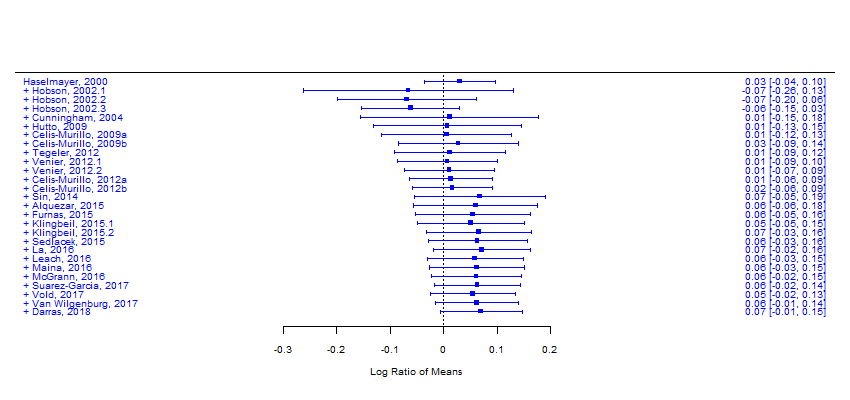
\includegraphics{Figures/Figure1.png}
\caption{Figure caption \label{figurelabel}}
\end{figure}


\end{document}
